\section{Explainability \& Alert Generation}
\subsection{Permutation Feature Importance Analysis}
To provide model interpretability, we evaluated empirical feature importance using permutation-based Macro F1 degradation on the hold-out test split. Features were permuted independently across 10 random iterations.

Fig. \ref{fig:feature_importance} illustrates the top feature importances for Informer. Engineered utilization indicators (\texttt{load\_utilization} and \texttt{demand\_utilization}) account for 74.29\% of the observed performance degradation when permuted, confirming that capacity stress variables are the primary drivers of model predictions. Electrical and asset telemetry (\texttt{transformer\_load}, \texttt{electricity\_demand}) account for 24.39\%, while meteorological variables (\texttt{temperature}, \texttt{rainfall}, \texttt{humidity}) contribute 1.97\%, and temporal flags account for 0.17\%. This confirms that environmental variables act as secondary stress modifiers operating through thermal indices ($\text{THI}$).

\begin{figure}[htbp]
\centering
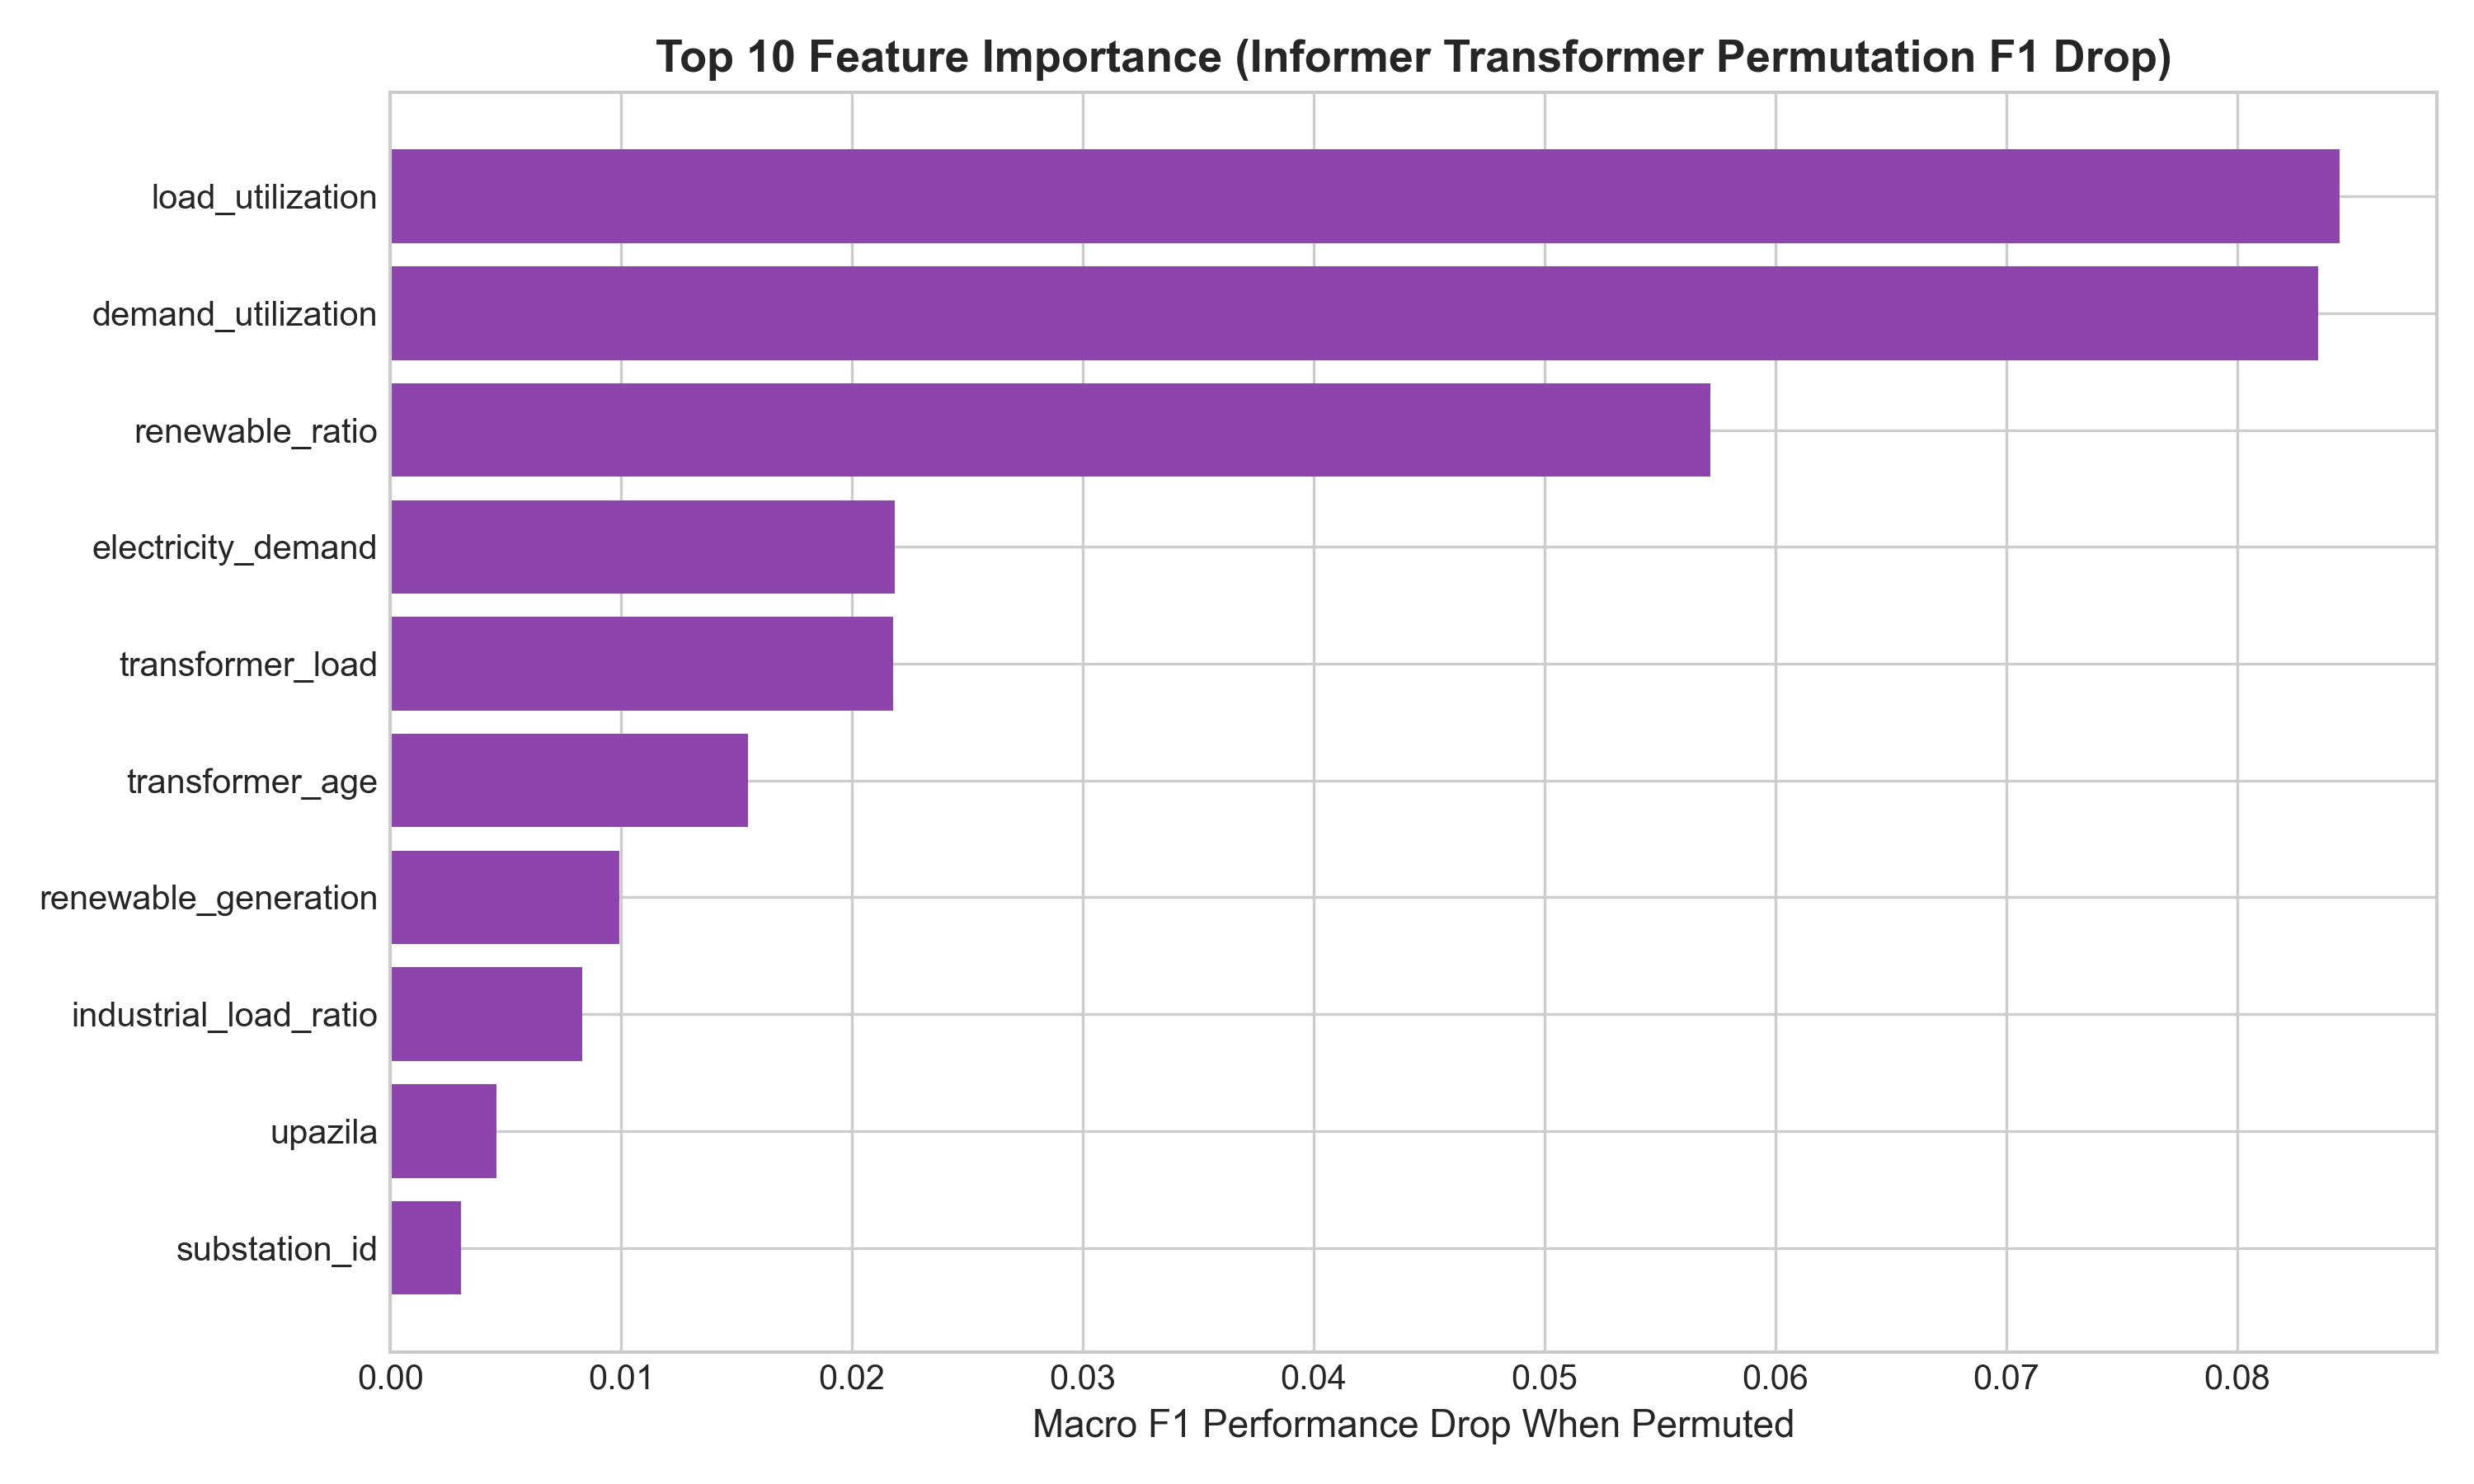
\includegraphics[width=0.88\linewidth]{figures/fig4_feature_importance.png}
\caption{Permutation Feature Importance Profile for the Informer Model.}
\label{fig:feature_importance}
\end{figure}

\subsection{Rule-Based Intelligent Alert Generation Engine}
To bridge deep learning probability outputs with utility control room operations, SmartGrid Sentinel routes model Softmax probabilities through a Rule-Based Natural Language Explanation Engine. Rather than providing uninterpretable raw attribution scores, the rule engine evaluates input telemetry against physical grid operating thresholds:

\begin{itemize}
    \item \textbf{GREEN (Normal Operation):} Predicted Risk = \texttt{Low}. Transformer loading is within safe operating bounds ($U_{\text{load}} \le 0.75$). Normal grid dispatch continues.
    \item \textbf{YELLOW (Warning Advisory):} Predicted Risk = \texttt{Medium}. Transformer loading is moderate ($0.75 < U_{\text{load}} \le 0.85$). The rule engine issues operator advisories: \textit{``Moderate capacity stress detected on feeder transformer. Dispatchers should monitor demand growth and notify industrial loads.''}
    \item \textbf{RED (Urgent Emergency):} Predicted Risk = \texttt{High}. Severe transformer loading ($U_{\text{load}} > 0.85$). The rule engine issues urgent advisories: \textit{``Electricity demand exceeds capacity thresholds ($U_{\text{load}} > 0.85$), indicating severe overload risk. Initiate precautionary load shedding on non-essential commercial feeders.''}
\end{itemize}

If environmental heat stress is high ($\text{THI} > 28.0$), the module appends: \textit{``Elevated environmental heat stress detected ($\text{THI} > 28.0$), accelerating transformer thermal degradation risks.''} These advisories are coupled with citizen recommendations (e.g., charging essential devices, throttling high-power cooling appliances).
